% (3-5 Seiten)
\section{Feature Evaluation}
\label{sec:FeatureEval}
This section evaluates the first and higher order features, which were described in Section \ref{sec:NEL}. The quality measures used to evaluate the features are again Precision $P$, Recall $R$ and the $F_{\beta}$-Score. Specifically, the $F_1$-Score is used, which is the harmonic mean of the Precision and the Recall and thus favors neither. The following sections will evaluate first the first order features, then the addition of all higher order features and finally every single higher order feature. Of these evaluations, the first and last ones are done with the leave-one-out strategy to avoid a time-consuming exhaustive grid search. In the case of the first order features, there is also no other way to evaluate the link score since it is equal for all feature entries generated from a single alias. The tests were done using a Random Forest classifier, which was trained as described in Section \ref{sec:ModelEval}. It was trained using these parameters: a maximum tree depth of 6, a maximum number of bins of 40 and with 20 trees.
% \begin{itemize}
% 	\item mit welchem Classifier getestet
% 	\item Parameter des Classifiers auch erwähnen
% 	\item erklären, warum keine exhaustive grid search (dauert zu lange)
% 	\item Training- und Testvorgang beschreiben (ist wie in der section davor)
% 	\item benutzen auch die gleichen Evaluierungsmaße
% 	\item eine "Control-Group" haben (mit allen Features)
% \end{itemize}

\subsection{First Order Features}
\begin{figure}[H]
	\centering
	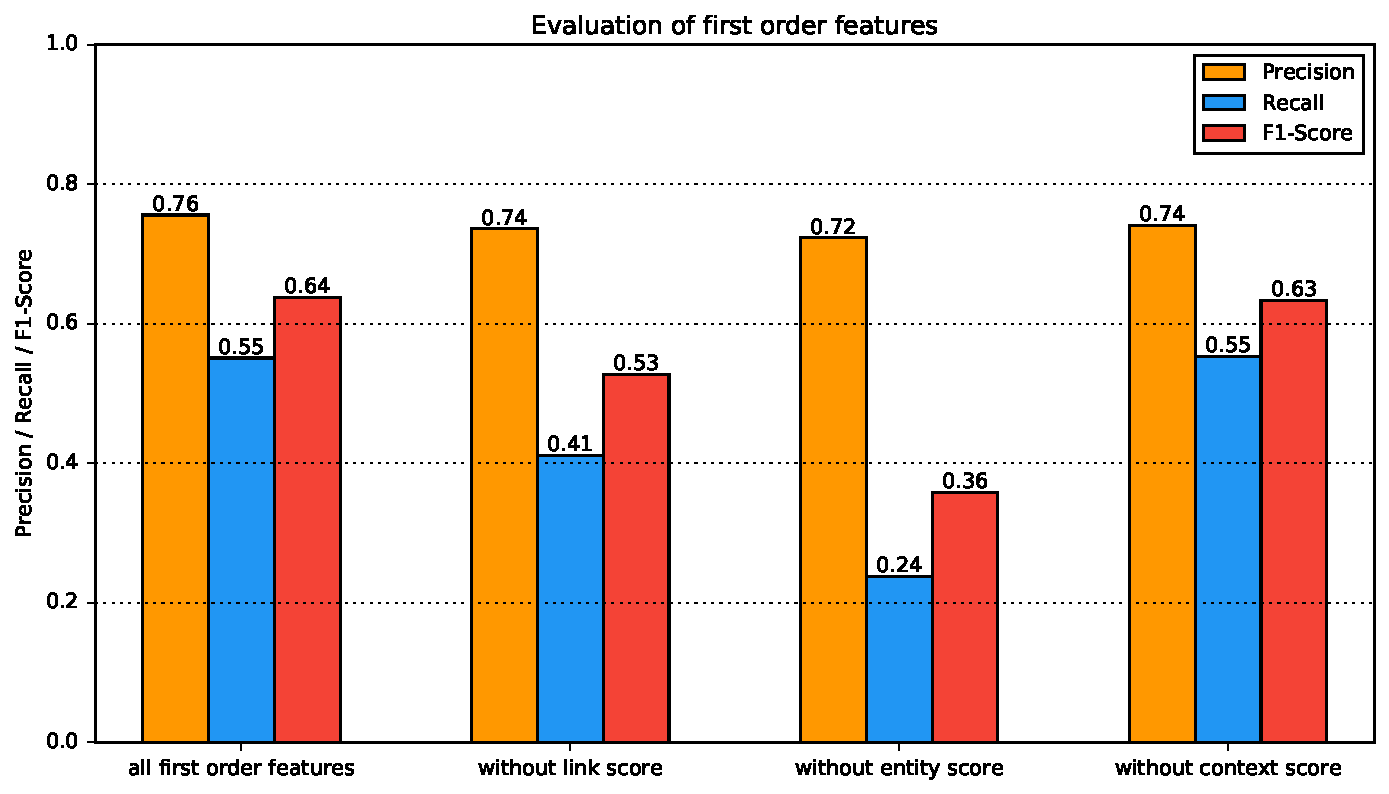
\includegraphics[width=\textwidth]{img/first_order_eval}
	\caption{Leave-one-out evaluation of the first order features.}
	\label{fo_eval}
\end{figure}
\begin{itemize}
	\item short description of first order features
	\item kurz beschreiben was man sieht (und alle first order als control group)
	\item link score:\\
		minimaler Precision drop und starker Recall drop\\
		variiert nicht bei den feature entries die für einen eintrag generiert wurden\\
		sagt hauptsächlich aus, ob dieser alias relevant ist oder nicht\\
		entsprechent fehlt bei manchen feature entries die aussage, dass dieses wort trotzdem wichtig ist\\
		deswegen wird es einfach nicht verlinkt (erklärt recall) anstatt auf die falsche entitaet zu verlinken (deswegen kaum precision drop)
	\item entity score:\\
		sichtbar dass wichtigstes feature überhaupt\\
		extrem starker recall abfall\\
		hat als feature den größten wertebereich (range)\\
		link score ist konstant für alle feature entries von einem alias\\
		context score hat relativ geringen wertebereich\\
		entsprechend sind viele aliase auch einfach gar nicht verlinkt, da der context score alleine nicht viel aussagt\\
		precision drop ist wieder minimal
	\item context score
		precision fällt auch minimal und recall ändert sich nicht\\
		dieses feature ist vor allem für die disambiguierung in nicht sicheren fällen\\
		entsprechend beeinflusst es vor allem die precision und erhöht die rate des richtigen disambiguierens
	\item abschließend die Rollen der Features dadurch validieren
\end{itemize}

\subsection{Higher Order Features}
\begin{figure}[H]
	\centering
	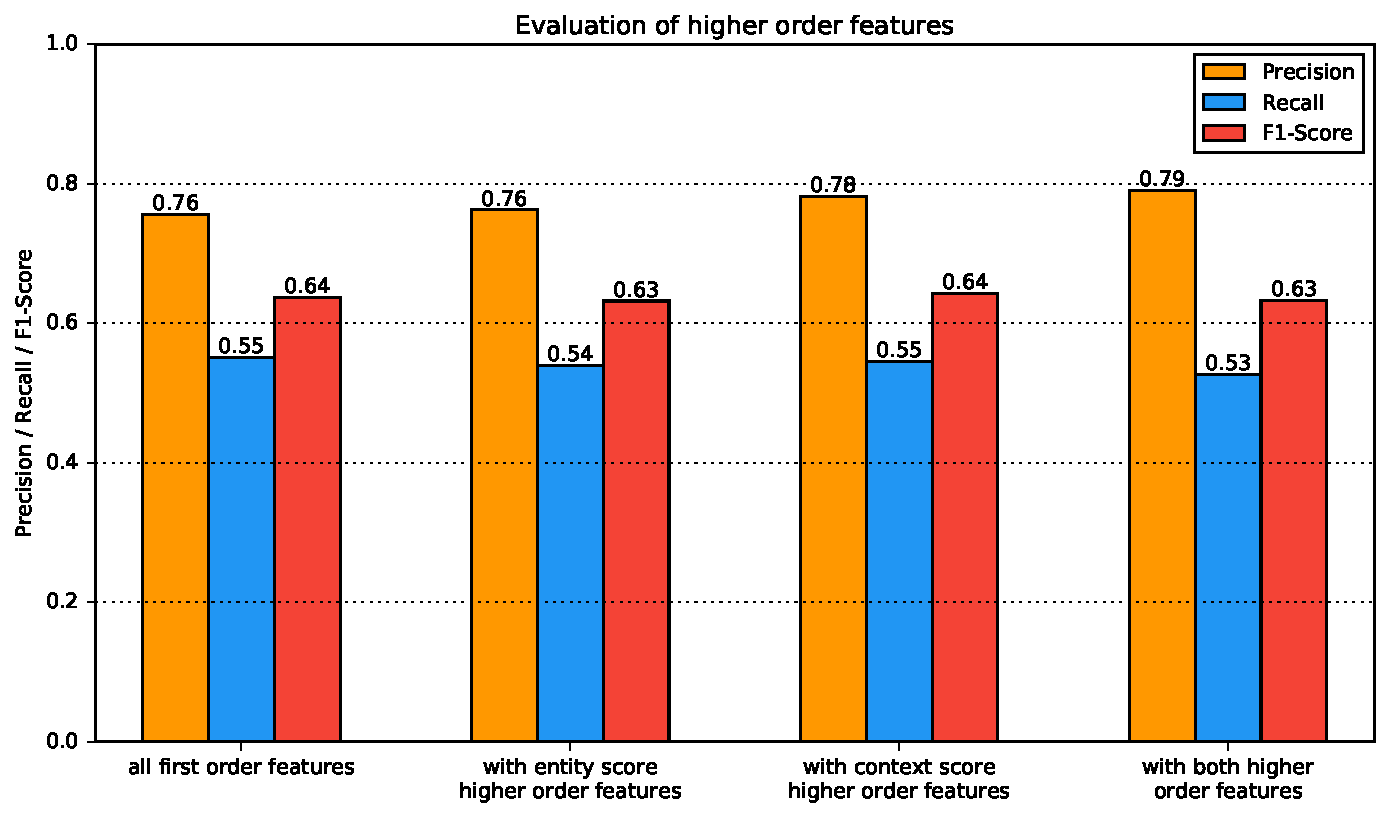
\includegraphics[width=\textwidth]{img/higher_order_eval}
	\caption{Evaluation of the higher order features.}
	\label{ho_eval_gen}
\end{figure}
\begin{itemize}
	\item kurz higher order features beschreiben
	\item kurz beschreiben was man sieht (und alle first order als control group)
	\item entity score higher order features\\
		minimale Verbesserung in Precision, die im Bild durch runden nicht zu sehen sind\\
		Recall fällt etwas\\
		nur kleine Änderungen, da der entity score alleine schon sehr Aussagekräftig ist\\
		higher order features helfen vor allem den Kontext zu den anderen Einträgen des gleichen alias darzustellen\\
		der ist oft durch den entity score selber auch schon gegeben
	\item context score higher order features\\
		Verbesserung der Precision ohne Fall des Recalls\\
		wieder: higher order features helfen vor allem den Kontext zu den anderen Einträgen des gleichen alias darzustellen\\
		bei context score hilft das wegen der relativ kleinen Werte und dem geringen Wertebereich eine vergleichsweise niedrige Zahl als wichtig einzustufen\\
		dadurch bessere disambiguierung
	\item beide higher order features\\
		erhöhen precision durch bessere disambiguierung\\
		verringern recall auch nur minimal\\
		der classifier wird etwas vorsichtiger, da z.B. bei 2 Kandidaten mit ähnlichen entity scores der classifier keinen nimmt weil der unterschied zu gering ist
	\item abschließend sagen dass die higher order features einen Leistungsanstieg bringen, dieser aber nur minimal ist
\end{itemize}

\begin{figure}[H]
	\centering
	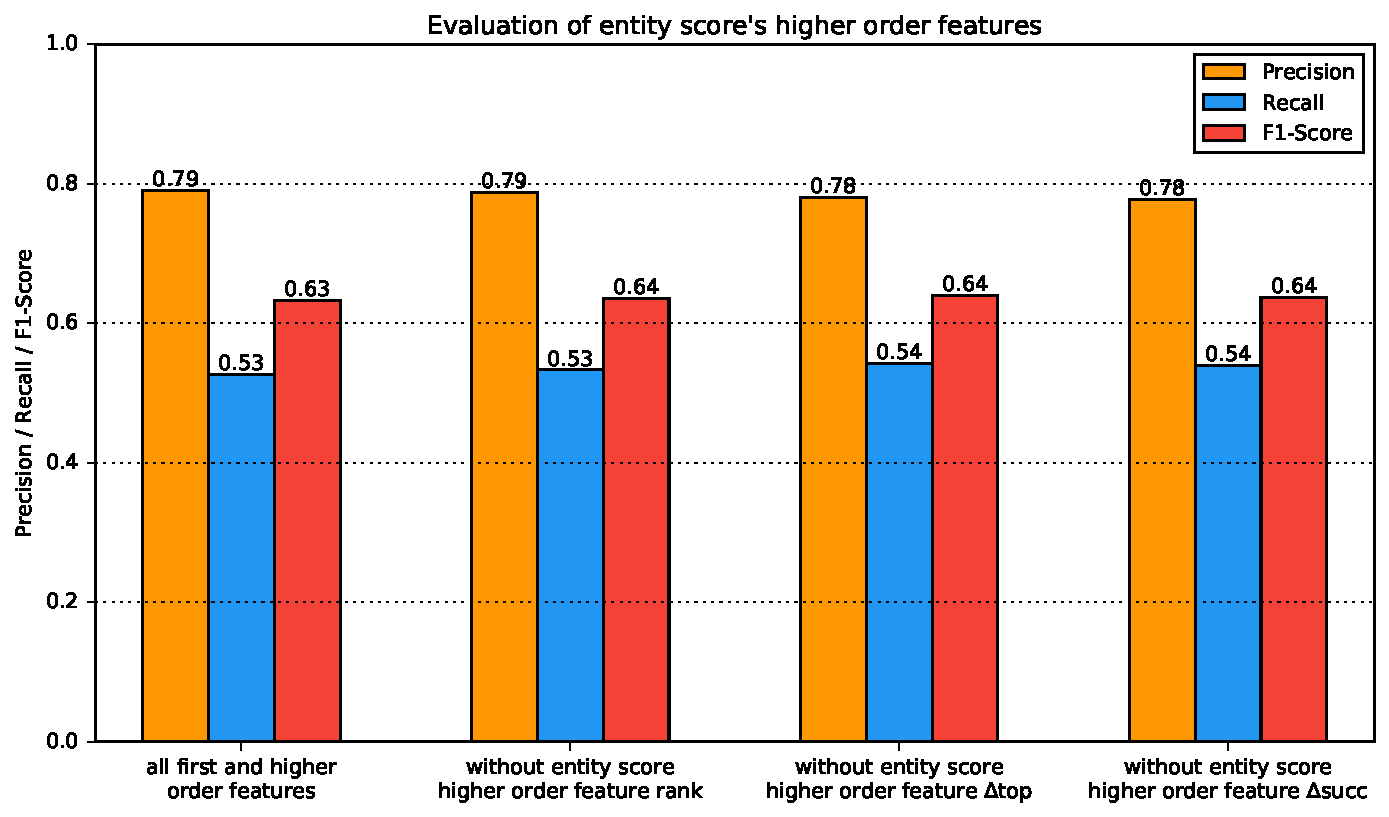
\includegraphics[width=\textwidth]{img/higher_order_eval_entity}
	\caption{Leave-one-out evaluation of the entity score's higher order features.}
	\label{ho_eval_entity}
\end{figure}
\begin{itemize}
	\item kurz beschreiben was man sieht (und alle first und higher order als control group)
\end{itemize}

\begin{figure}[H]
	\centering
	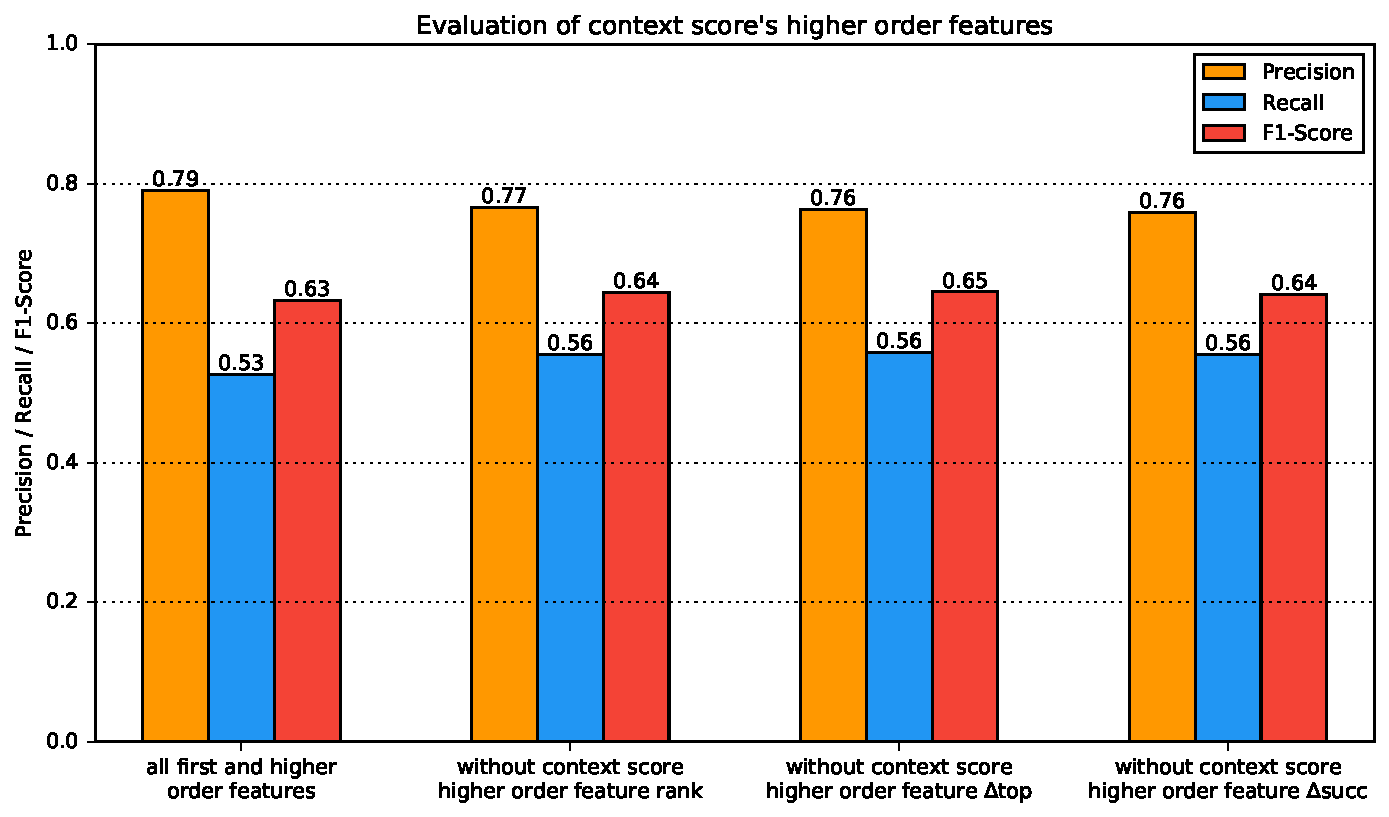
\includegraphics[width=\textwidth]{img/higher_order_eval_context}
	\caption{Leave-one-out evaluation of the context score's higher order features.}
	\label{ho_eval_context}
\end{figure}
\begin{itemize}
	\item kurz beschreiben was man sieht (und alle first und higher order als control group)
\end{itemize}












